\documentclass[titlepage]{article}
\usepackage{array}
\usepackage{enumerate}
\usepackage{graphicx}
\usepackage{listings}
\usepackage{tabularx}

\begin{document}

\author{Stevan Stanisic and Santana Mach}
\title{COMP 8505 - Final Project \\ Rootkit \\ Testing Documents}
\date{Dec 05, 2011}
\maketitle{}

\tableofcontents
\pagebreak

\section{Introduction}

The 

\section{Usage Instructions}

Placeholder.

\section{Testing Design}

\begin{tabularx}{\textwidth}{|c|X|X|X|c|}
\hline
\textbf{\#} & \textbf{Description} & \textbf{Tools Used} & \textbf{Expected Result} & \textbf{Pass}\\
\hline
1 & Validate IP \& UDP checksums & bkdoor\newline Wireshark & Checksums are correct in Wireshark & Yes\\
\hline
2 & Backdoor channel via UDP source port. & bkdoor\newline Wireshark & Signature \& \newline encrypted data in the source port. & Yes\\
\hline
3 & Backdoor channel via NTP Ref ID. & bkdoor\newline Wireshark & Signature \& \newline encrypted data in the reference clock id. & Yes\\
\hline
4 & Backdoor channel via DNS ID. & bkdoor\newline Wireshark & Signature \& \newline encrypted data in the transaction id. & Yes\\
\hline
5 & Basic commands & bkdoor & Receive output of commands from server & Yes\\
\hline
6 & Exfiltrate file. & bkdoor\newline echo & File is exfiltrated from the server. & Yes\\
\hline
7 & Changing watch\newline directory. & bkdoor & Execute new server with new watching directory & Yes\\
\hline
\end{tabularx}

\section{Testing Data}

\subsection{Test \# 1 - Checksums}

\begin{figure}[htb]                                                                       
  \begin{center}
    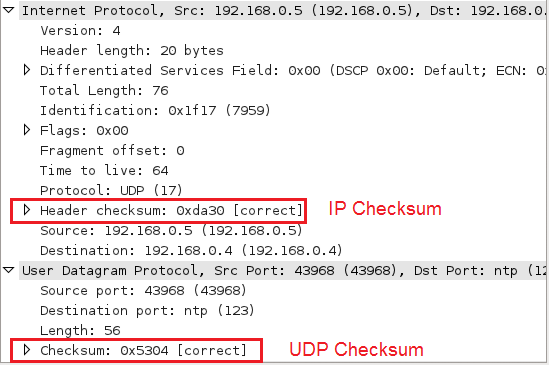
\includegraphics[width=0.9\textwidth]{Pictures/Checksum.png}
  \end{center}
  \caption{IP and UDP Checksums}
  \label{fig:checksums}
\end{figure}

\clearpage

\subsection{Test \# 2 - UDP Channel}

\begin{figure}[htb]                                                                       
  \begin{center}
    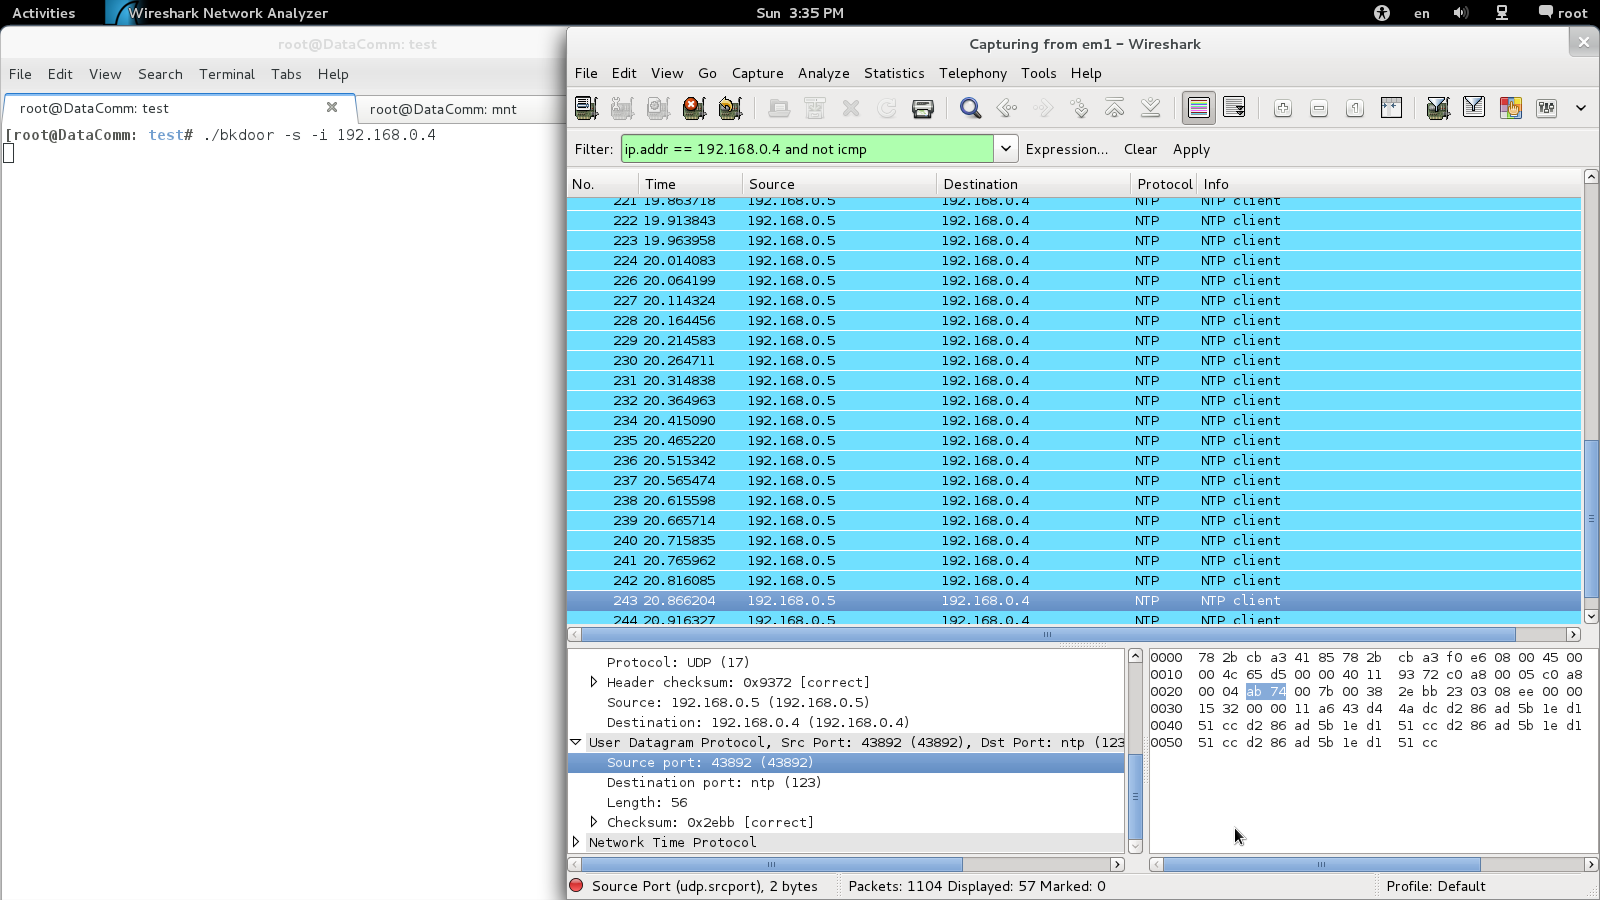
\includegraphics[width=0.9\textwidth]{Pictures/UDP_SIG.png}
  \end{center}
  \caption{UDP Channel Signature}
  \label{fig:udp_sig}
\end{figure}

\clearpage

\subsection{Test \# 3 - NTP Channel}

\begin{figure}[htb]                                                                       
  \begin{center}
    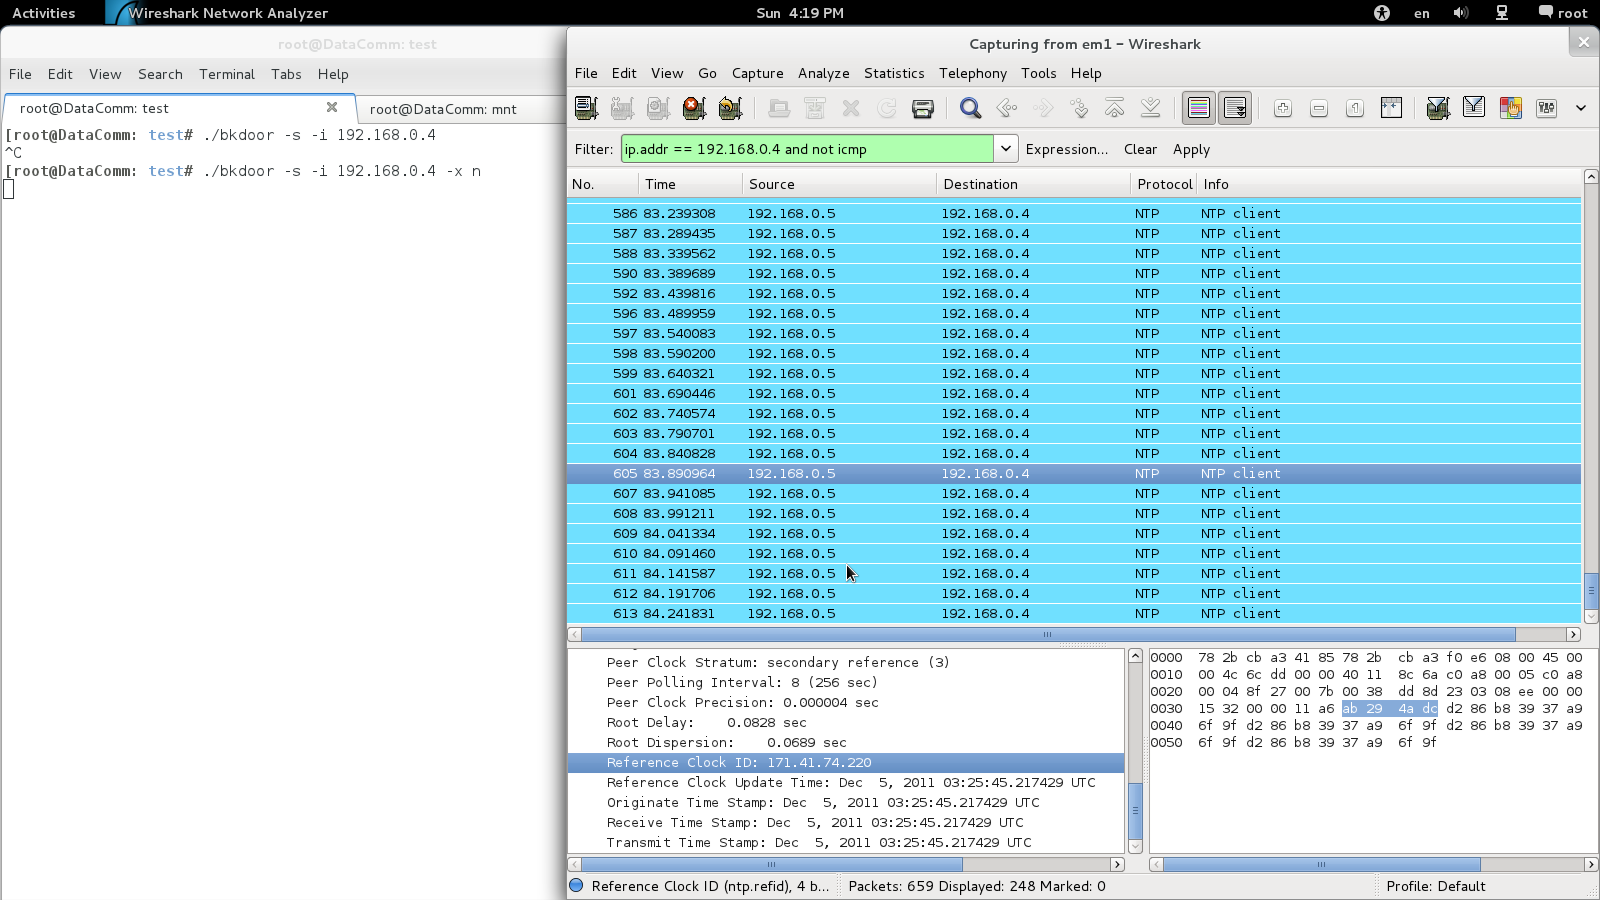
\includegraphics[width=0.9\textwidth]{Pictures/NTP_SIG.png}
  \end{center}
  \caption{NTP Channel Signature}
  \label{fig:ntp_sig}
\end{figure}

\clearpage

\subsection{Test \# 4 - DNS Channel}

\begin{figure}[htb]                                                                       
  \begin{center}
    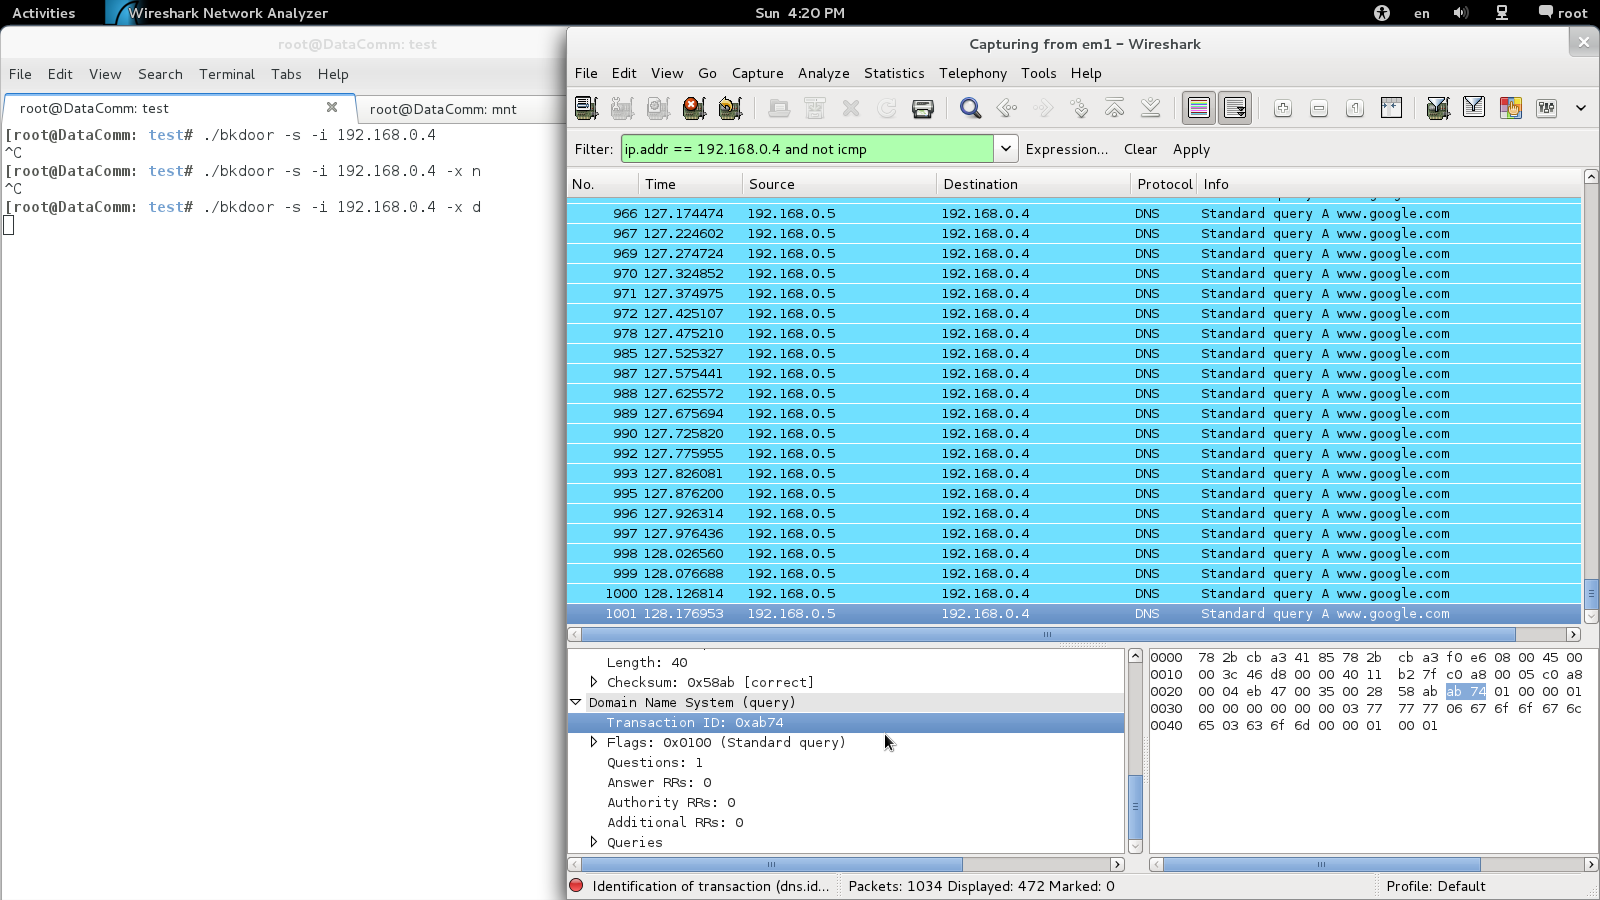
\includegraphics[width=0.9\textwidth]{Pictures/DNS_SIG.png}
  \end{center}
  \caption{DNS Channel Signature}
  \label{fig:dns_sig}
\end{figure}

\clearpage

\subsection{Test \# 5 - Basic Commands}

\begin{figure}[htb]                                                                       
  \begin{center}
    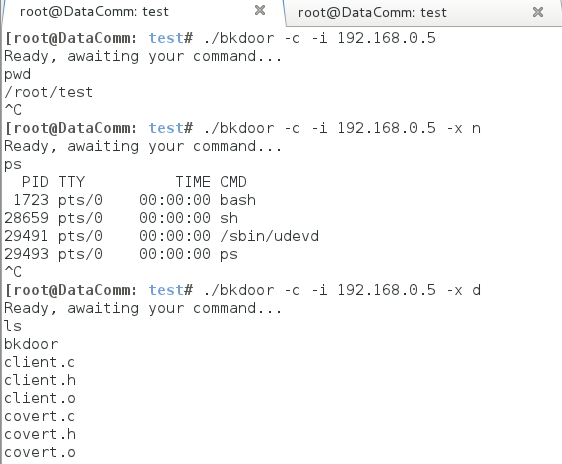
\includegraphics[width=0.9\textwidth]{Pictures/Commands.png}
  \end{center}
  \caption{Output of Commands}
  \label{fig:commands}
\end{figure}

\clearpage

\subsection{Test \# 6 - Exfiltration}

\begin{figure}[htb]                                                                       
  \begin{center}
    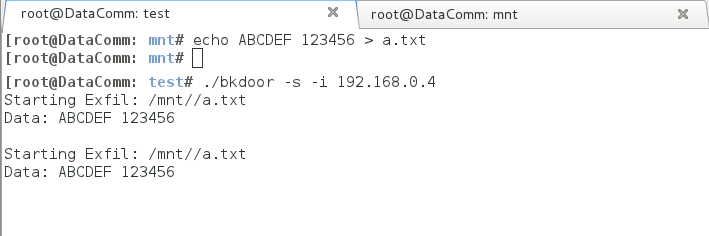
\includegraphics[width=0.9\textwidth]{Pictures/Exfiltration.png}
  \end{center}
  \caption{File Exfiltration}
  \label{fig:exfiltration}
\end{figure}

\clearpage

\subsection{Test \# 7 - Changing Watch Directory}

\begin{figure}[htb]                                                                       
  \begin{center}
    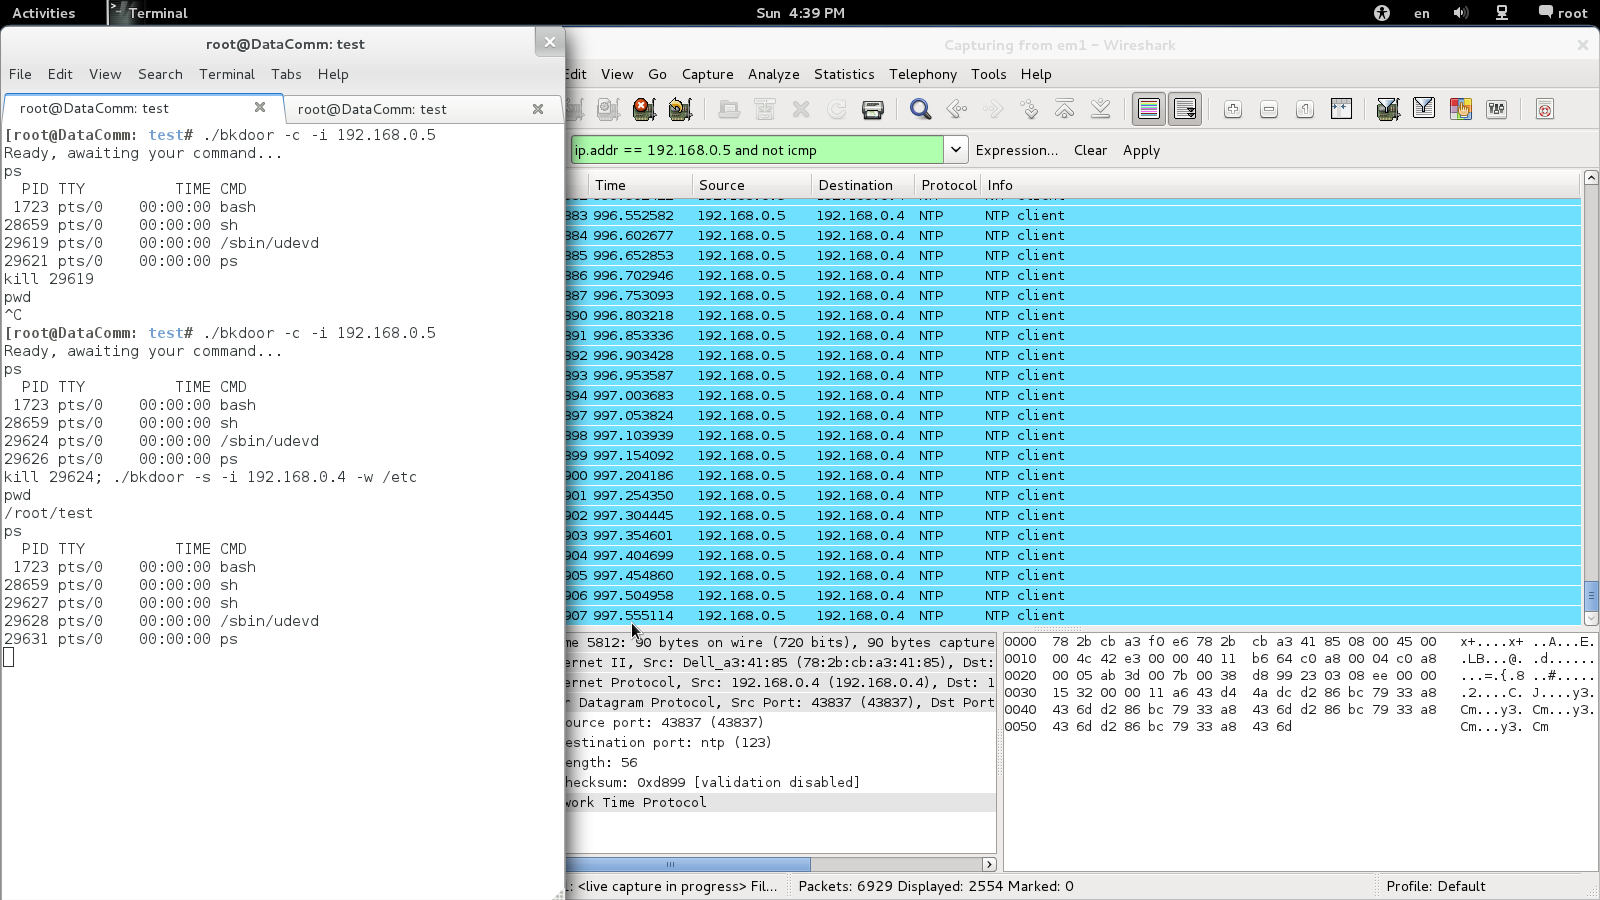
\includegraphics[width=0.9\textwidth]{Pictures/Watch.png}
  \end{center}
  \caption{Example of Watch Directory}
  \label{fig:watch}
\end{figure}

\clearpage

\section{Conclusion}

Placeholder.

\end{document}
